\Introduction
\label{chap:introduction}

L'informatique graphique, branche du domaine de l'informatique, est l'étude de la création d'images numériques par ordinateur~\cite{poinssac_infographie_1994}. C'est un domaine à l'intersection de plusieurs disciplines, comme l'informatique, les mathématiques, la physique, l'optique, la biologie, et d'autres encore. L'informatique graphique trouve ses applications dans de nombreux autres domaines~\cite{ekaran_when_2021}, notamment celui du divertissement. Un défi de l'informatique graphique qui se dresse depuis ses débuts est celui de la création de contenu, car c'est un processus long et coûteux. Dans la figure~\ref{fig:hades} par exemple, le personnage, les bâtiments et leur architecture, la rivière et les effets de lumières sont tous des éléments créés par une équipe d'artistes. Il existe diverses méthodes pour créer du contenu~\cite{juegoadmin_why_2023}, dont plusieurs comme le modelage 3D, qui demandent beaucoup de temps de travail aux artistes. De nos jours en particulier, il y a une demande croissante pour des univers virtuels de plus en plus grands et détaillés~\cite{imam_open_2022}. Les méthodes traditionnelles de création de contenu, par le pur travail manuel des artistes, sont de moins en moins viables en raison de la quantité de contenu nécessaire à créer pour remplir ces univers~\cite{freiknecht_survey_2017}. Il est important de mettre au point des méthodes plus automatisées pour permettre une création plus rapide et moins coûteuse.

\bigskip

\begin{figure}[!h]
    \centering
    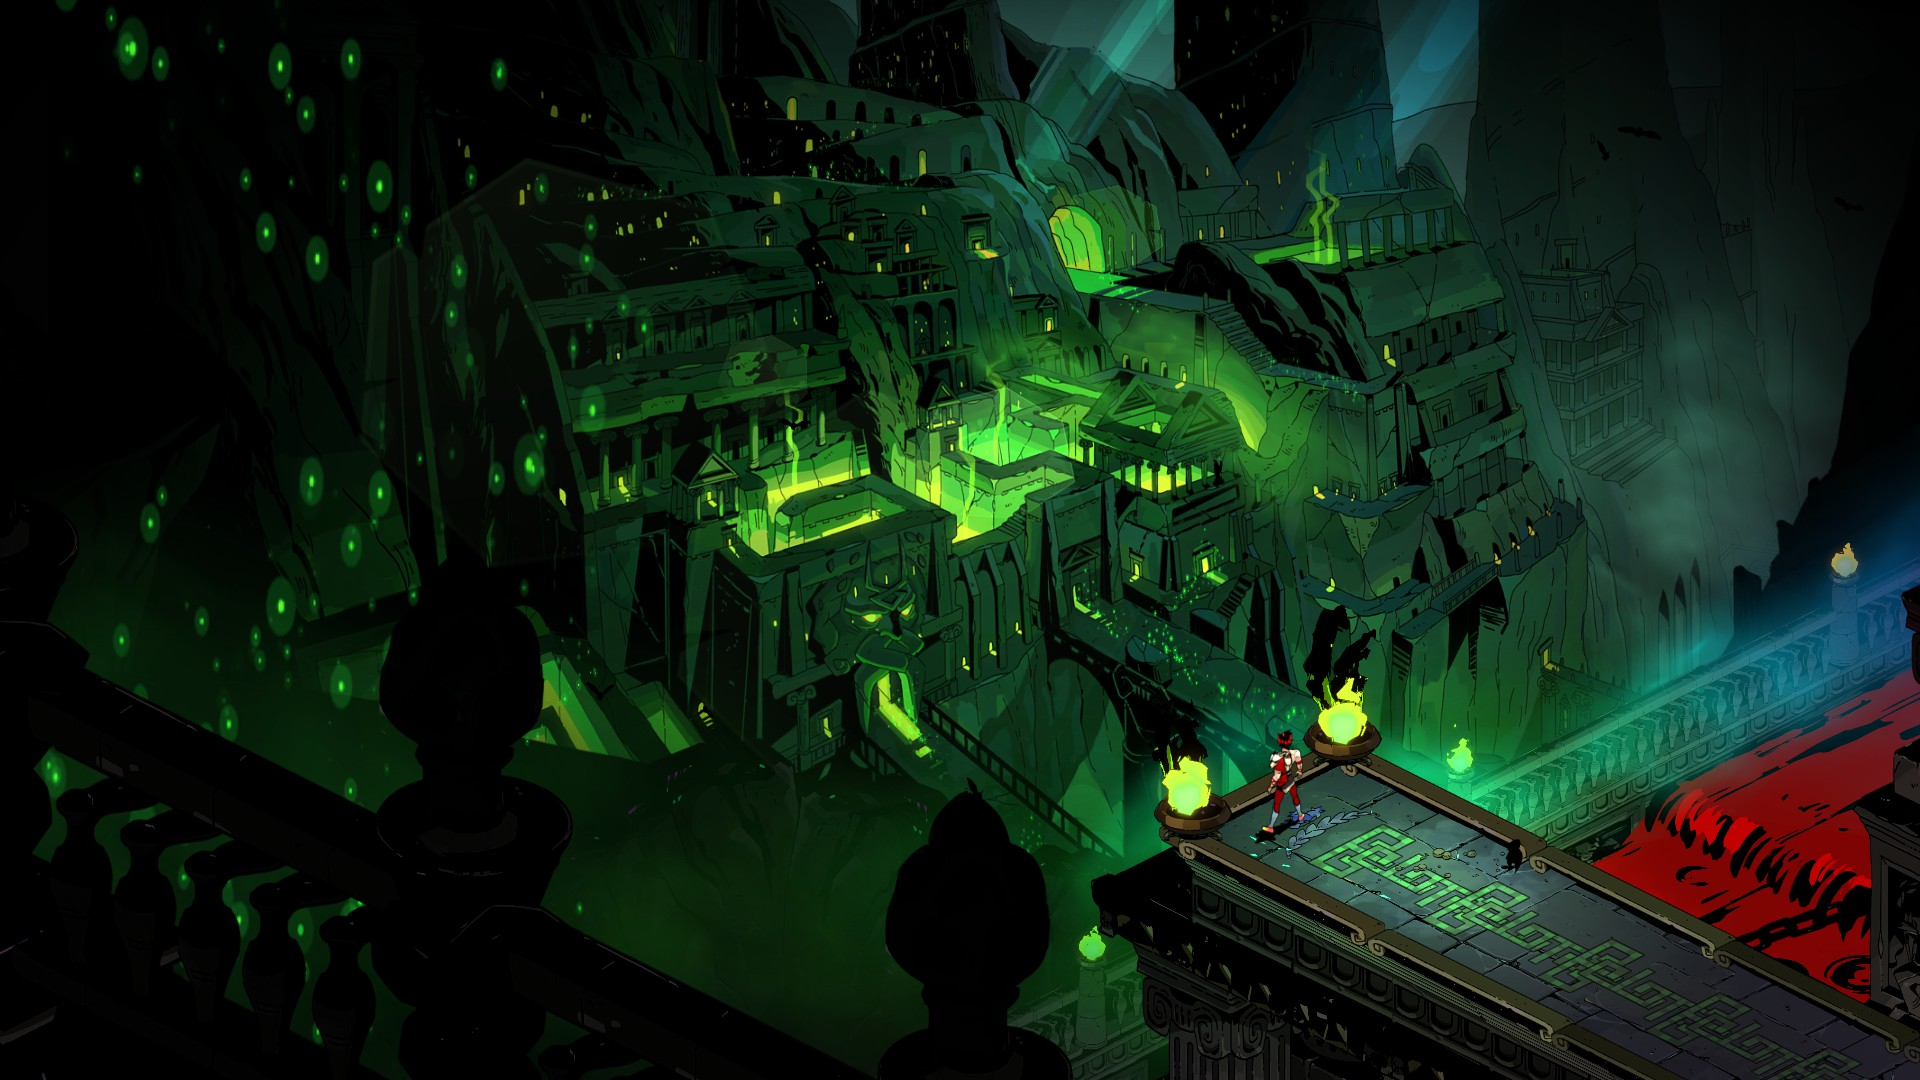
\includegraphics[width=.85\textwidth]{contenu/resources/images/hades}
    \caption[\textit{Hades} (2018), Supergiant Games]{\textit{Hades} (2018), Supergiant Games~\cite{supergiant_hades_2018}}
    \label{fig:hades}
\end{figure}

% TODO HEREE

Dans ce contexte de méthodes automatisées, la génération procédurale est un procédé utilisé pour produire toutes sortes de ressources numériques~\cite{smelik_survey_2014}. Elle est en particulier utilisée pour synthétiser l'apparence visuelle des différents composants des scènes virtuelles~\cite{alessio_procedural_2021}. En combinant des méthodes algorithmiques avec de l'aléatoire, il est possible de générer des cartes de texture qui servent à habiller les mondes virtuels. Une carte de texture désigne une image qui est appliquée sur une surface pour lui donner un aspect visuel dans le but d'accentuer l'immersion des utilisateurs. Différentes textures nécessitent différentes méthodes de synthèse pour être générées. Certains genres de textures sont encore difficilement réalisables avec les méthodes existantes~\cite{lutz_cyclostationary-gaussian_2021}. C'est dans cette perspective que s'inscrit ce travail de recherche, qui a pour but d'approfondir notre compréhension des éléments qui constituent la structure d'une image. La compréhension d'une image et de ces éléments est le sujet d'un autre domaine, le traitement du signal (une image est un signal 2D). Le traitement du signal est un sous-domaine du génie électrique qui étudie la manipulation et l'interprétation des signaux. Nebeker définit le traitement du signal comme étant [...] l'ensemble des changements appliqués aux signaux dans le but d'améliorer leur transmission et utilisation. (traduction libre)~\cite{nebeker_fifty_1998}. Quand le signal étudié est une image, le domaine est appelé traitement ou analyse d'image. Afin obtenir une meilleure compréhension de la structure d'une image, ce travail explore l'analyse locale multirésolution et son application à la synthèse de texture procédurale. L'analyse locale multirésolution est un outil du domaine de l'analyse d'image et est détaillée dans la suite de ce manuscrit au chapitre~\ref{chap:chapitre1}.

\section{Monde virtuel}

Dans le cadre de l'informatique graphique, un monde virtuel est une méthode de représentation de scènes au moyen d'un support numérique. Une scène est une collection d'objets numériques qui interagissent entre eux. Il existe trois sortes d'objets numériques qui composent une scène : de la géométrie, des lumières et des caméras. Avec des algorithmes dits de rendu, un monde virtuel peut être converti en image. Les mondes virtuels sont utilisés dans de nombreux domaines~\cite{magnenat-thalmann_introduction_1986}, comme :

\begin{itemize}
    \item le domaine du divertissement, pour les jeux vidéo (l'industrie du jeu-vidéo est un des principaux acteurs des avancées en graphisme) ;
    \item le domaine de l'animation, pour les films d'animation ou les effets spéciaux de films ;
    \item le domaine médical, pour des outils de visualisation de l'anatomie humaine ou de formation en réalité virtuelle ;
    \item le domaine de l'ingénierie, pour aider à la conception d'objets (Conception Assistée par Ordinateur) ou de bâtiments (architecture) ;
    \item le domaine militaire, pour faire des simulations de situations ou des entraînements au combat.
\end{itemize}

\subsection*{Types de rendu}

La visualisation de scènes virtuelles s'opérationnalise au travers d'un logiciel dit moteur de rendu utilisant divers algorithmes pour fonctionner~\cite{sherman_chapter_2003}. Un moteur de rendu traite une scène en différentes étapes dans le but de créer une visualisation de cette scène, appelée rendu de la scène~\cite{pharr_physically_2023}. Il existe plusieurs méthodes de rendu qui implémentent différents algorithmes pour produire différentes visualisations d'une scène. Pour exécuter leurs calculs, les logiciels de rendu s'appuient sur les capacités des cartes graphiques ({\it Graphics Processing Unit} ou GPU). Ces dernières sont des processeurs hautement parallèles et spécialisés dès leur fabrication pour des calculs graphiques~\cite{das_history_2016}.

\bigskip

\begin{figure}[h]
    \centering
    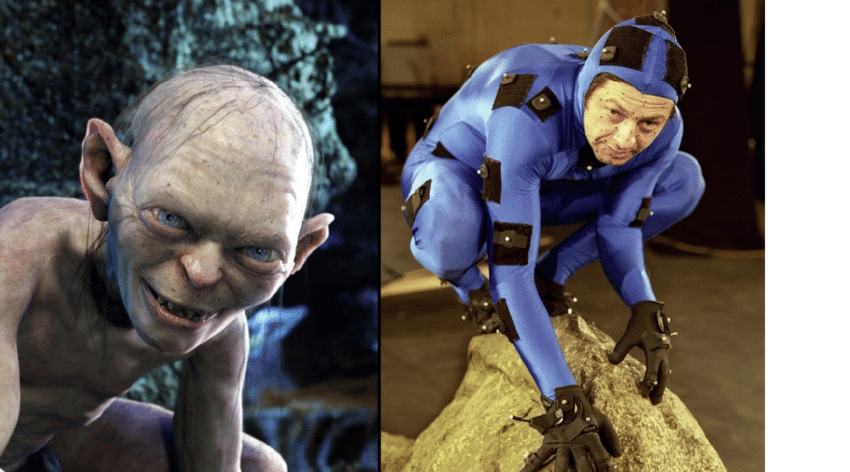
\includegraphics[width=.65\textwidth]{contenu/resources/images/gollum}
    \caption[{\it Gollum} (2002), {\it Le Seigneur des Anneaux : Les Deux Tours}]{{\it Gollum}, personnage complètement généré par image de synthèse par rendu hors-ligne. {\it Le Seigneur des Anneaux : Les Deux Tours}, Peter Jackson~\cite{jackson_lord_2002}. Image par Mou~\cite{mou_keyframe_2018}.}
    \label{fig:gollum}
\end{figure}

Les méthodes de rendu peuvent être séparés en deux grandes catégories : le rendu hors-ligne et le rendu en temps-réel. Le rendu hors-ligne désigne les algorithmes qui font la visualisation de scènes non interactives, où il n'est pas possible de contrôler les interactions entre les éléments de la scène. Les films d'animation ou les effets spéciaux de films~\ref{fig:gollum} sont des exemples de rendus fait hors-ligne. L'utilisation de méthodes de rendu hors-ligne est en fait devenu une norme dans l'industrie cinématographique~\cite{media_history_2021}, car elle permet la création de scènes qu'il serait impossible de tourner à l'aide de caméras traditionnelles. À l'inverse, lors d'un rendu en temps-réel, une personne utilisatrice a un contrôle sur la scène qui est rendue pendant qu'elle est rendue. Le déplacement d'un personnage dans un jeu-vidéo, la manipulation d'un modèle de pont dans un logiciel d'architecture et l'affichage d'objets dans une application de réalité augmentée sont tous des exemples de rendus en temps-réel. Une même scène peut être rendue avec plusieurs méthodes de rendu, la visualisation finale sera alors différente à chaque fois. Une scène rendue en temps-réel d'une part et hors-ligne d'autre part, est montrée à la figure~\ref{fig:zero-day}. Les enjeux et contextes des rendus hors-ligne et en temps-réel diffèrent. Le travail présenté dans ce manuscrit s'intéresse aux méthodes de rendu en temps-réel. Dans la méthode proposée, bien qu'une partie de préparation des données soit nécessaire, le rendu final se fait en temps-réel. Les problématiques et solutions concernant le rendu hors-ligne ne sont donc pas abordées dans ce travail.

\bigskip

\begin{figure}[h]
    \centering
    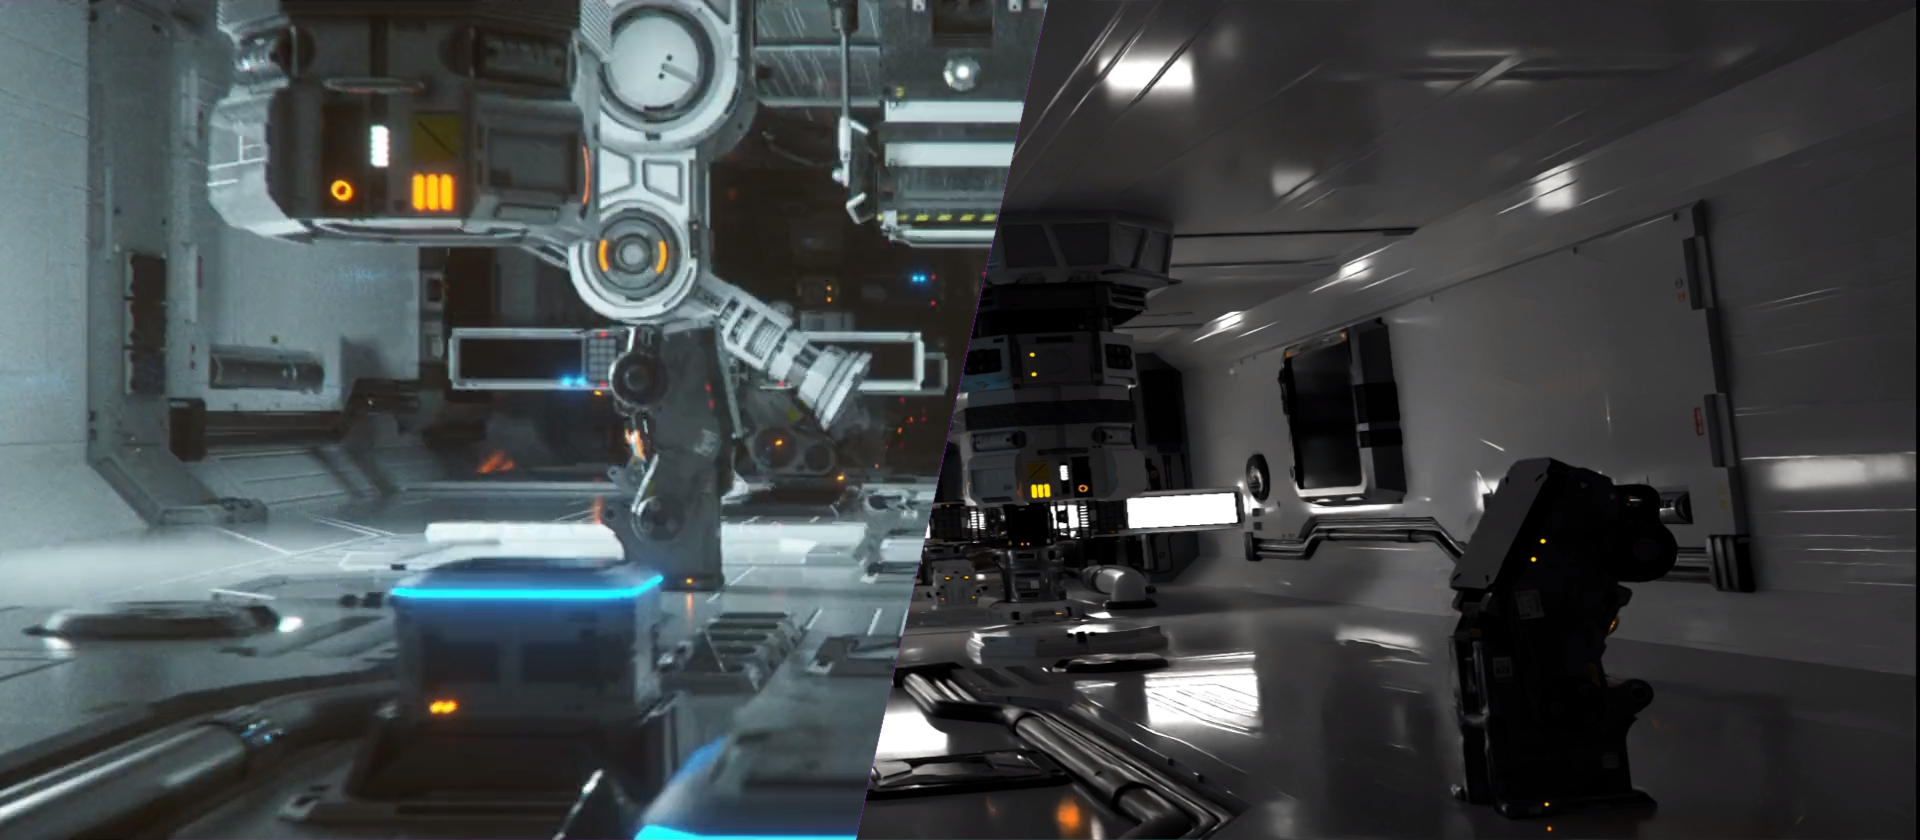
\includegraphics[width=\textwidth]{contenu/resources/images/zero_day_comparison}
    \caption[{\it Zero-Day} (2015), BEEPLE]{{\it Zero-Day} (2015), BEEPLE. À gauche rendu original hors-ligne, à droite rendu temps-réel par tracé de chemins, NVIDIA~\cite{winkelman_zero-day_2019}}
    \label{fig:zero-day}
\end{figure}

Une méthode de rendu en temps-réel doit répondre à certaines contraintes dues à la nature interactive de la scène. Le rendu de la scène ne peut pas se faire en avance, car la scène est modifiée pendant l'utilisation. Le rendu doit être assez rapide pour afficher les images assez vite de telle sorte que le flux soit continu à l'œil humain. L'industrie cinématographique utilise un standard de 24 images par secondes pour l'enregistrement de films~\cite{deguzman_why_2023}. Pour un rendu en temps-réel, les applications visent des objectifs d'au moins 30 ou 60 images par secondes, afin que le contrôle utilisateur soit confortable~\cite{janzen_is_2014}. Les algorithmes utilisés doivent ainsi être conçus pour s'exécuter avec moins de temps, moins de ressources de calcul, et moins d'espace mémoire disponible.

\subsection*{Maillage}

Pour manipuler une scène virtuelle, il est nécessaire d'avoir une représentation des éléments qui la composent. Une représentation est une manière technique de décrire et stocker les données d'une scène. Il y a deux façons de représenter une géométrie dans un monde virtuel. Les représentations continues, comme les surfaces implicites, se rapprochent au mieux des formes des objets du monde réel, mais sont difficiles à créer. Les représentations discrètes, comme les maillages, approximent les représentations continues par des ensembles de polygones~\cite{coons_surfaces_1967}, souvent des triangles. Les polygones qui forment un maillage sont définis explicitement par des données géométriques, notamment les positions des sommets et les sommets des faces. La figure~\ref{fig:procedural-mesh} montre les polygones qui composent un modèle de terrain. Dans ce travail, seuls les maillages seront utilisés. Les maillages sont des structures habituelles dans les mondes virtuels.

\begin{figure}[h!]
    \centering
    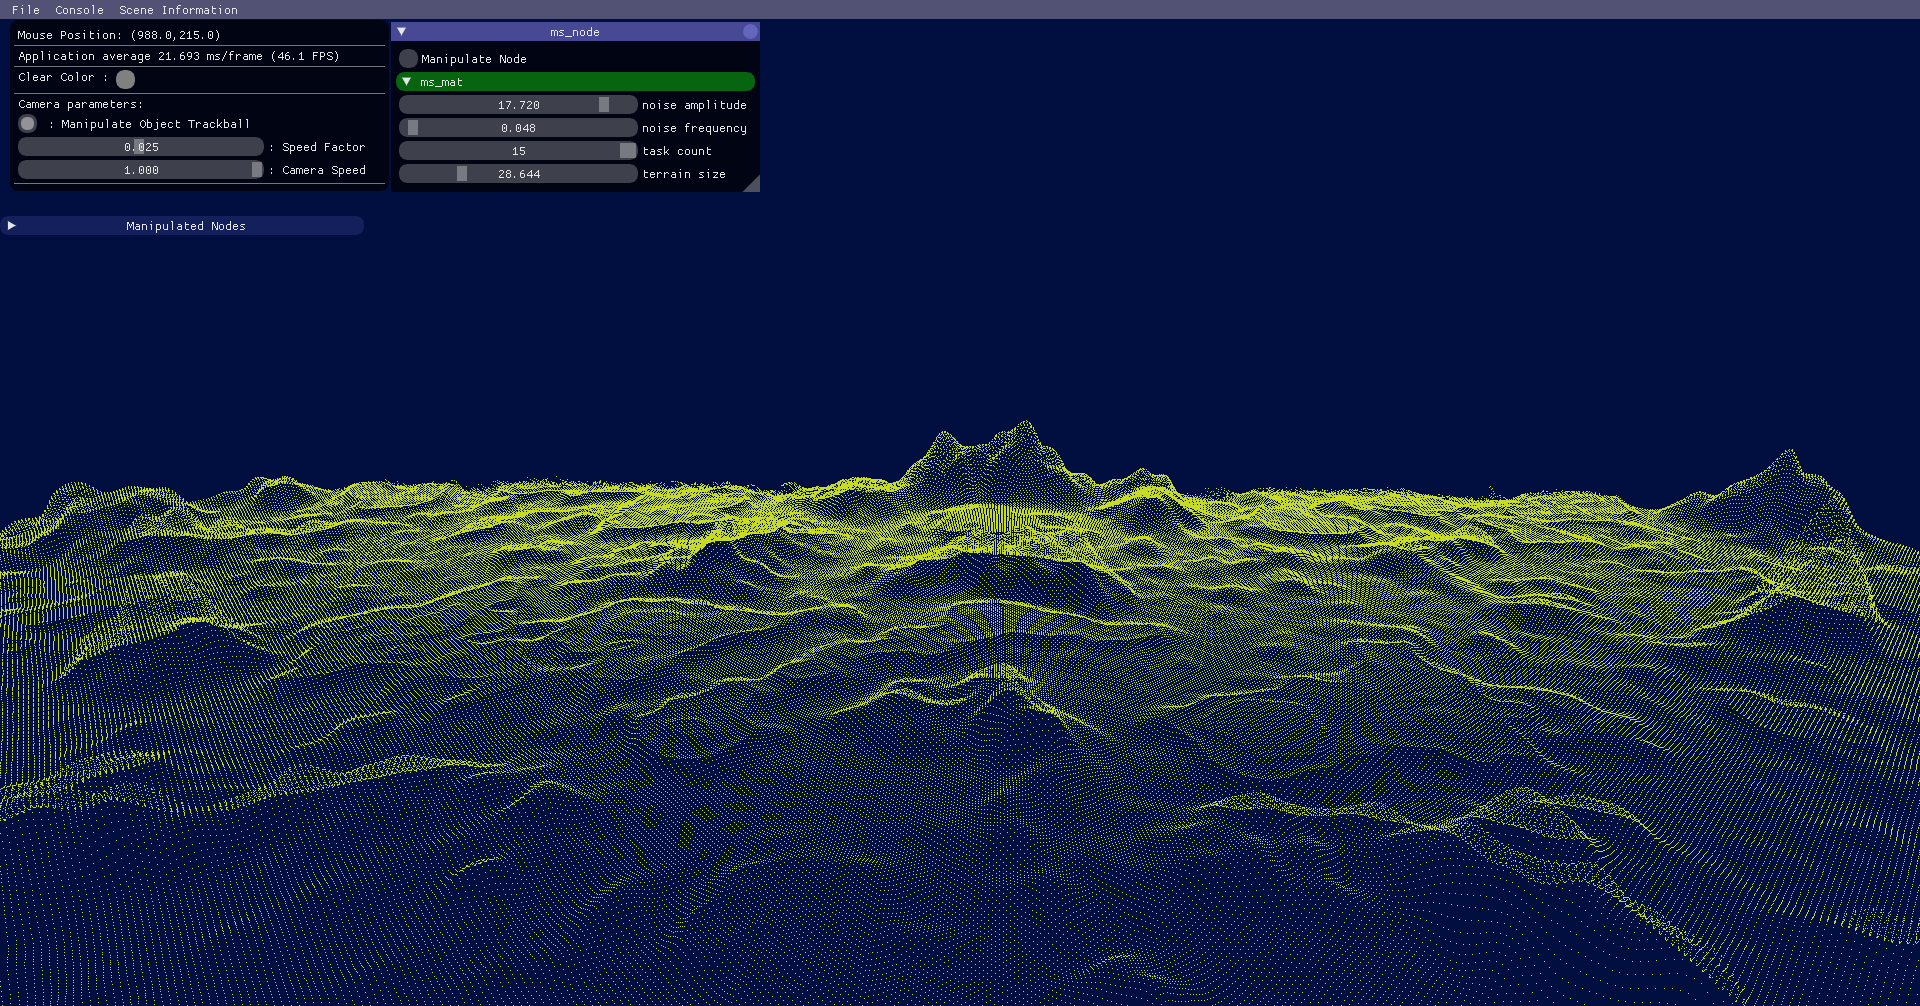
\includegraphics[width=\textwidth]{contenu/resources/images/full_terrain}
    \caption{Maillage d'un terrain généré procéduralement}
    \label{fig:procedural-mesh}
\end{figure}

\section{Texture}

\subsection*{Plaquage de texture}

Le maillage utilisé pour représenter une géométrie est une approximation. Pour affiner la géométrie, ou lui attribuer une apparence, il est possible d'utiliser des textures. Une texture est une fonction d'un espace de coordonnées, habituellement à deux ou trois dimensions, à valeurs dans un espace quelconque qui représente les différents attributs possibles de la texture. Les dimensions de l'espace d'arrivée sont appelées canaux de la texture. Les textures représentent généralement la couleur d'une surface, ou d'autres grandeurs physiques comme la profondeur ou l'élévation, qui servent au rendu de la géométrie à laquelle est associée la texture. En fonction du modèle de rendu choisi pour la scène, différentes textures sont nécessaires. Le format de rendu physique réaliste ({\it Physically Based Rendering} ou PBR), standard de l'industrie~\cite{hoffman_siggraph_2010}, nécessite typiquement cinq cartes de texture~\cite{pharr_physically_2023} : l'albedo (ou couleur), mais aussi la normale, la hauteur, la rugosité et l'occlusion ambiante.

\bigskip

\begin{figure}
    \centering
    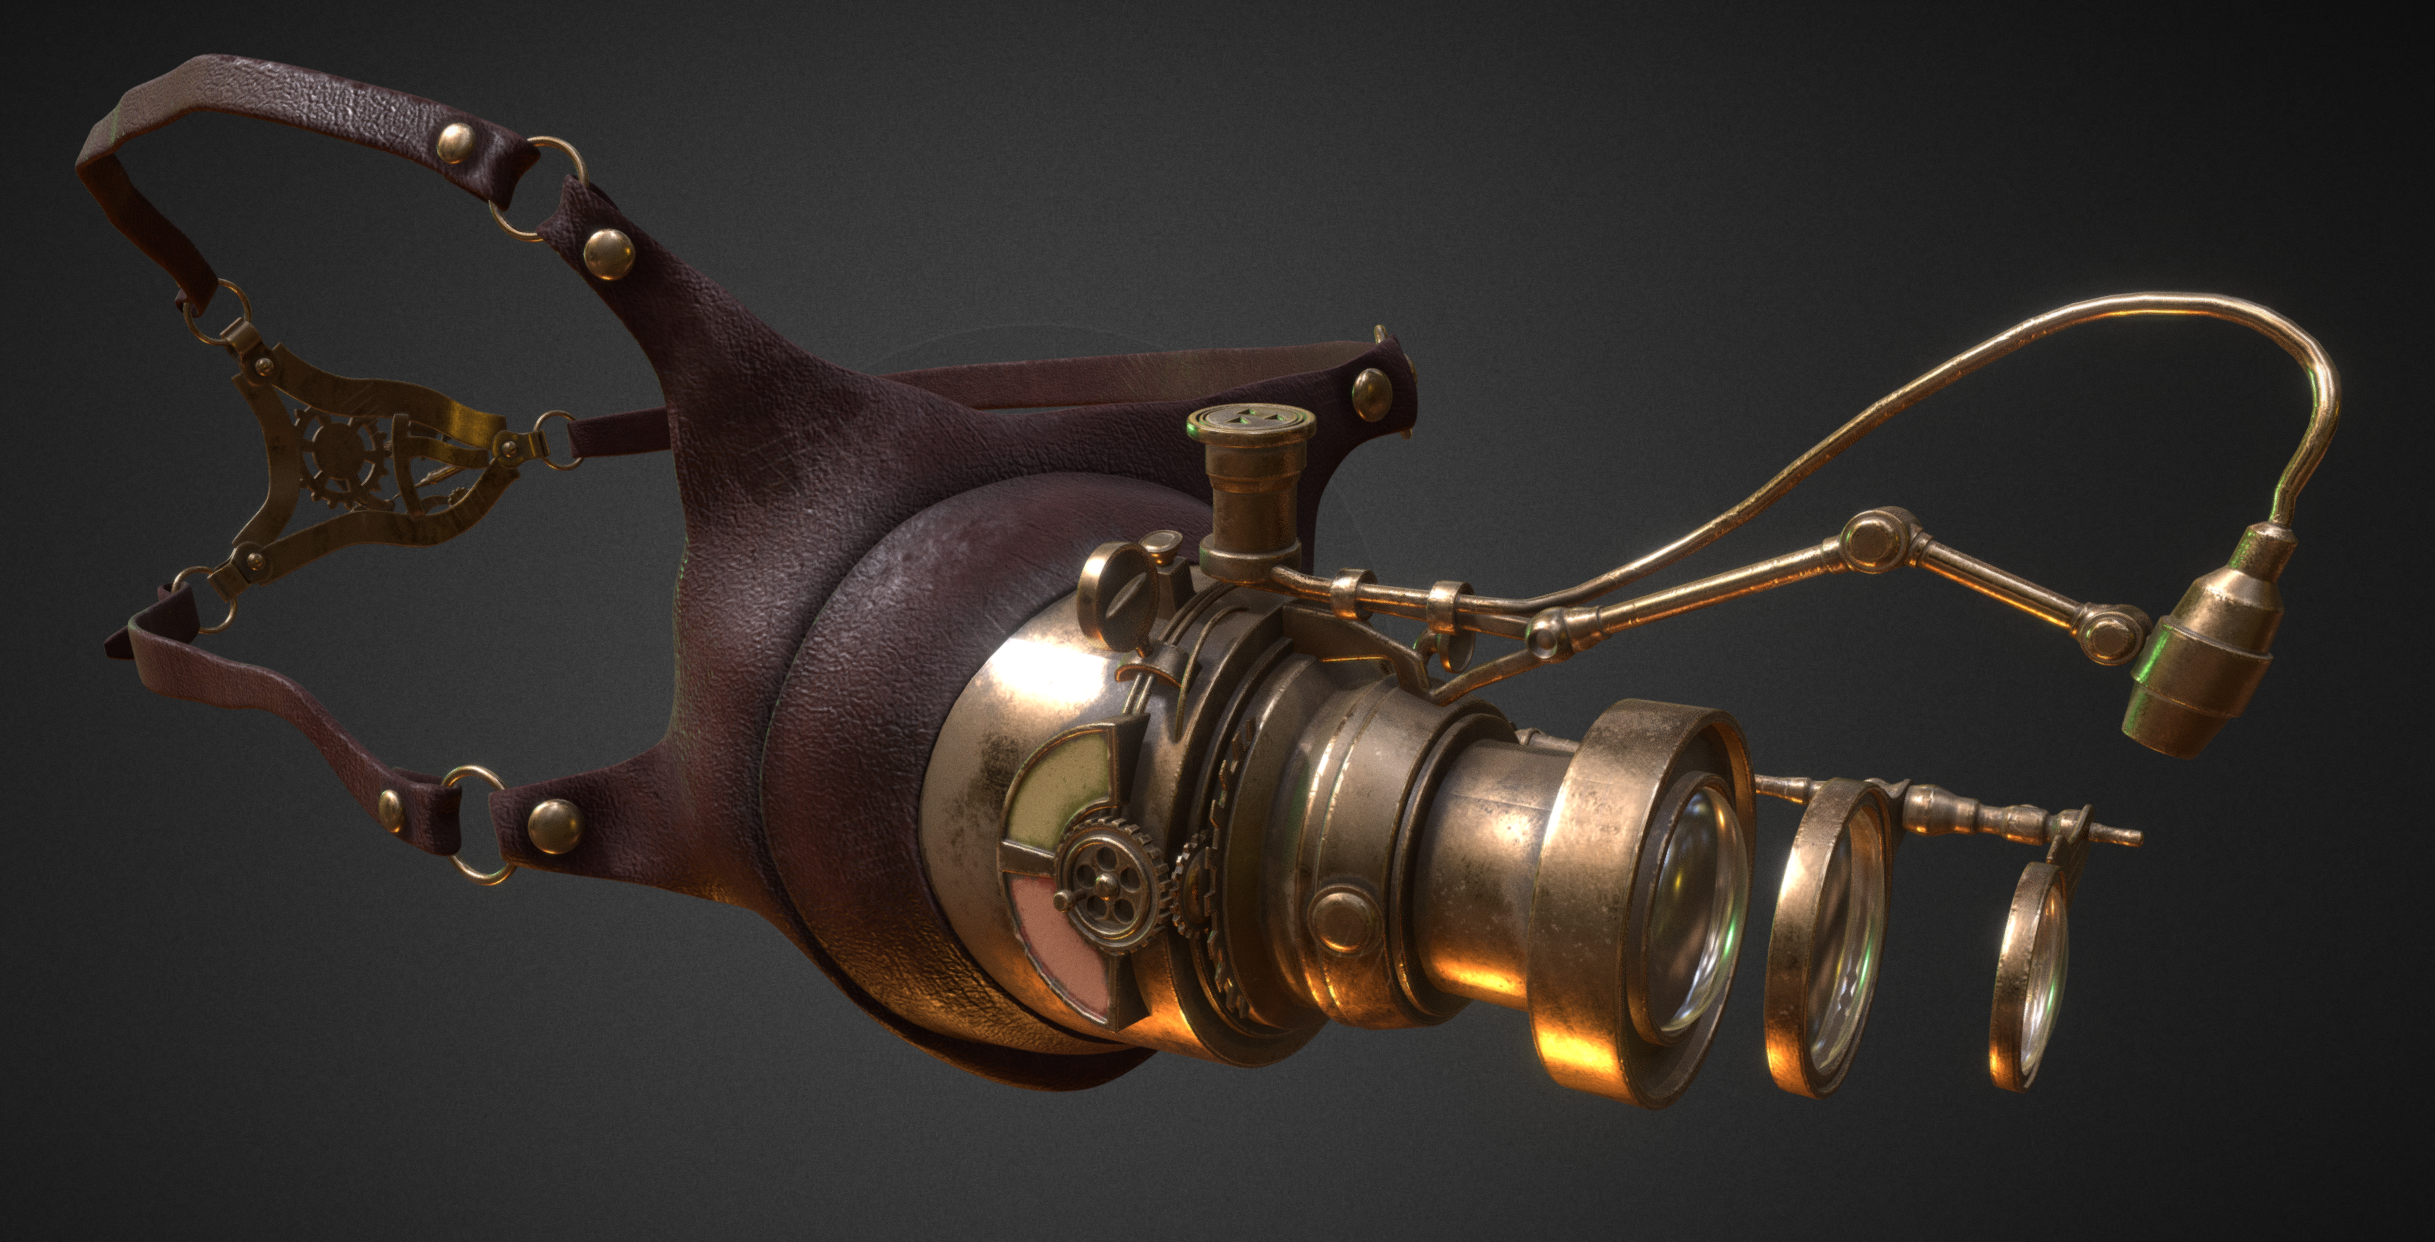
\includegraphics[width=.65\textwidth]{contenu/resources/images/mutli-material-object}
    \caption[Rendu d'un objet comportant plusieurs matériaux]{Plusieurs matériaux différents sont utilisés pour le rendu de cet objet~\cite{lepkarepka_steampunk_2021}}
    \label{fig:multi-material}
\end{figure}

La méthode de travail usuelle en industrie consiste à regrouper ces différentes textures, ainsi que le modèle d'éclairage, dans une ressource dite matériau. Les objets d'une scène sont composés de plusieurs matériaux, qui présentent chacun des propriétés physiques différentes. Dans la figure~\ref{fig:multi-material} par exemple, la lunette a un harnais en cuir, un objectif en métal et des lentilles en verre. Pour créer leurs scènes, les artistes façonnent leurs objets en commençant par la géométrie, avant de créer (ou réutiliser) différents matériaux pour habiller leurs objets.

\bigskip

Il existe deux méthodes classiques de stockage pour une texture : procédurale ou discrète. Une texture procédurale est représenté sous une forme fonctionnelle, à l'aide d'équations ou de procédures. Une texture discrète, quant à elle, est stockée comme une image numérique, c'est-à-dire un tableau discret et fini de données. La représentation procédurale, dont un exemple est donné à la figure~\ref{fig:perlin-noise}, présente plusieurs avantages par rapport à la représentation discrète :

\begin{itemize}
    \item la compacité : pour stocker une texture procédurale, il suffit de stocker les fonctions ou chaines d'instructions qui la définissent. Une texture procédurale n'occupe donc que très peu d'espace en mémoire.
    \item la taille : une texture procédurale est définie comme une fonction sur un espace de paramètre. Une texture procédurale est donc intrinsèquement infinie.
    \item la résolution : une texture procédurale est une fonction continue au sens mathématique. Il est possible de connaître la valeur exacte d'une texture procédurale en n'importe quel point de l'espace de coordonnées en l'évaluant en ce point.
\end{itemize}

Les textures procédurales ont cependant des désavantages. Certaines apparences souhaitées sont difficilement exprimables de manière fonctionnelle. Une expression fonctionnelle peut aussi être difficile à manipuler pour des artistes, puisqu'il faut ajuster des paramètres et modifier l'apparence de manière indirecte. De plus, l'expression d'une texture procédurale est parfois complexe et peut être un enjeu pour la synthèse en temps-réel. Il arrive que la fonction ou suite d'instructions qui définissent une texture procédurale sont si longs à exécuter que le budget de temps pour le rendu de l'image est dépassé. Une texture qui fait dépasser le budget temps du rendu n'est pas viable.

\bigskip

\begin{figure}[h]
    \centering
    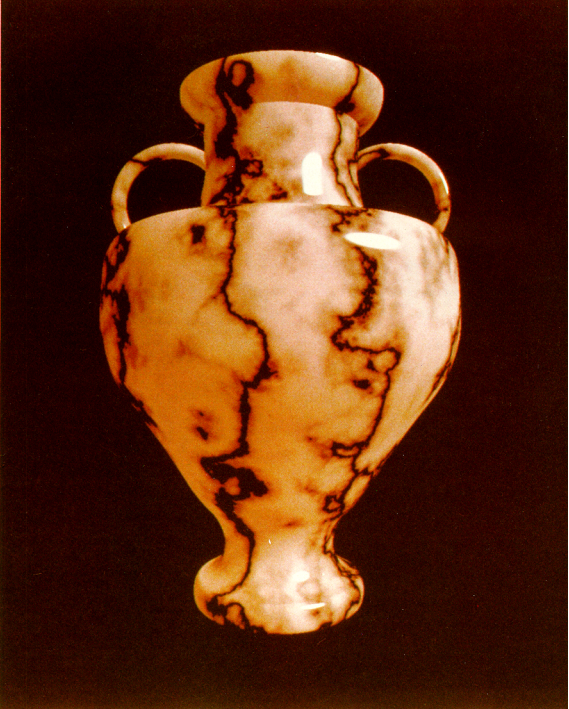
\includegraphics[width=.5\textwidth]{contenu/resources/images/perlin-noise}
    \caption[Bruit de Perlin]{La notion de texture procédurale est introduite par Ken Perlin en 1985 avec son bruit de Perlin~\cite{perlin_image_1985}.}
    \label{fig:perlin-noise}
\end{figure}

Résoudre les problématiques des textures procédurales est un enjeu de l'informatique graphique. Obtenir de nouvelles apparences, avoir un meilleur contrôle par les artistes et une évaluation plus rapide sont des sujets constamment explorés dans le domaine~\cite{heitz_high-performance_2018, tricard_procedural_2019, lutz_cyclostationary-gaussian_2021, baldi_differentiable_2023}. Le sujet présenté dans ce manuscrit s'inscrit dans la problématique de l'agrandissement du champ des apparences représentables par texture procédurale.

\subsection*{Échantillonnage}

Le processus utilisé traditionnellement pour le rendu en temps-réel est appelé le pipeline graphique de rastérisation. Dans ce pipeline, la scène rendue est projetée sur le plan image, qui est une représentation virtuelle de l'écran. La géométrie est ensuite divisée en petits éléments de surface appelés fragments, durant l'étape éponyme de rastérisation. La figure~\ref{fig:rasterization} montre comment un triangle est rastérisé dans le pipeline traditionnel. Les fragments sont les éléments atomiques du pipeline de rastérisation : ce sont les plus petits éléments indivisibles manipulés. Au terme du processus de rendu, un fragment est soit défaussé car non visible dans l'image finale, soit donné une couleur et affiché. Un fragment affiché à l'écran est appelé un pixel (mot-valise de \textit{Picture Element}). L'ensemble des pixels forme l'image rendue.

\begin{figure}[h]
    \centering
    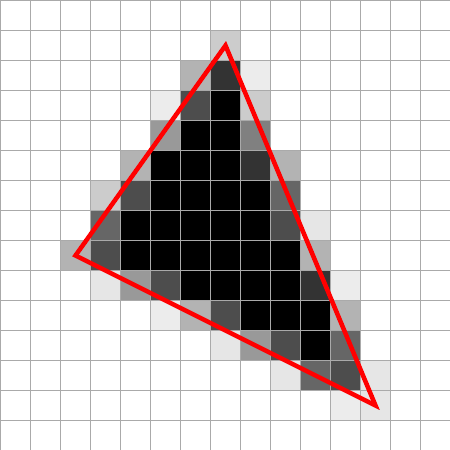
\includegraphics[width=.55\textwidth]{contenu/resources/images/rasterization}
    \caption[Rastérisation d'un triangle]{Un triangle (rouge) rastérisé (noir). Crédit à \textit{Wojciech mula} pour l'image.}
    \label{fig:rasterization}
\end{figure}

\bigskip

\begin{figure}
    \centering
    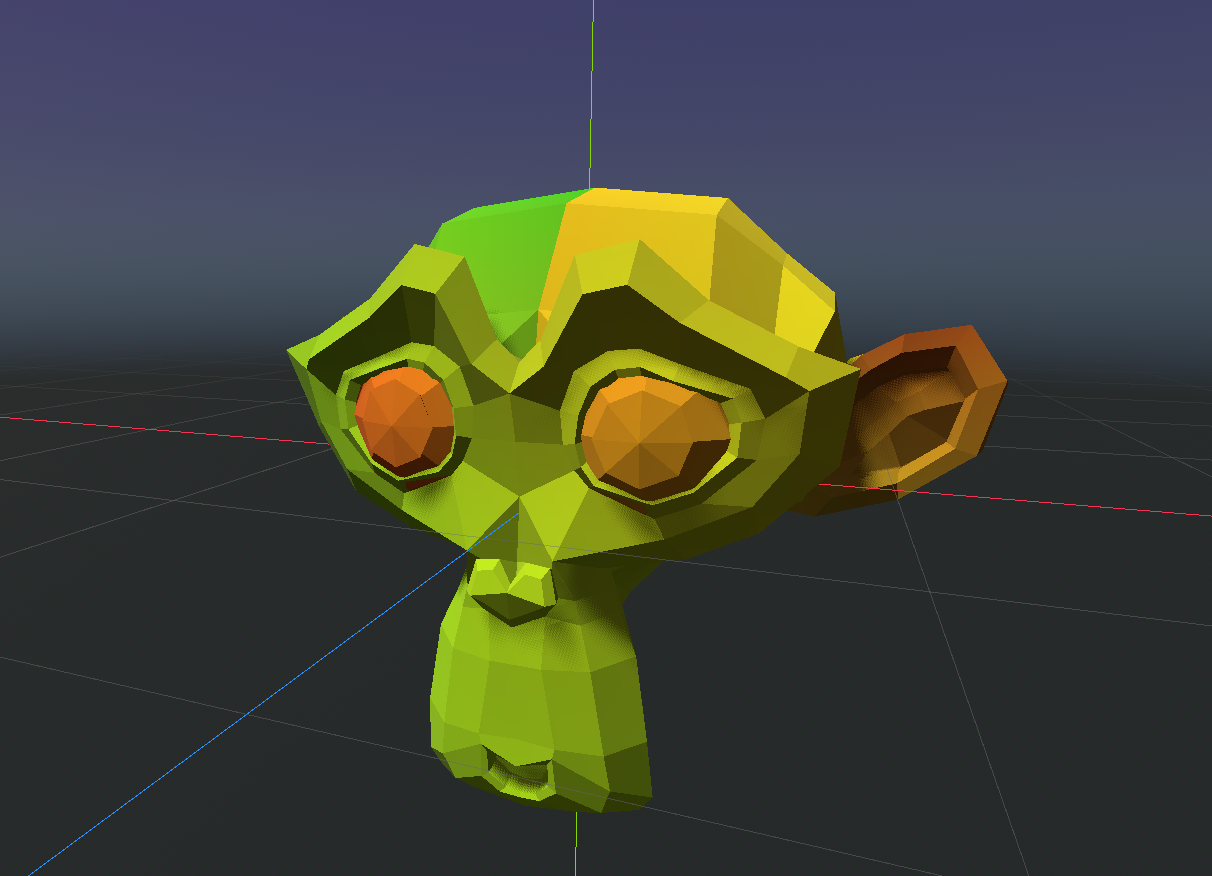
\includegraphics[width=.55\textwidth]{contenu/resources/images/uv_suzanne}
    \caption[Coordonnées UV du modèle Suzanne]{Visualisation des coordonnées UV de Suzanne~\cite{overbruggen_suzanne_2002}, modèle 3D de référence du logiciel Blender}
    \label{fig:uv-suzanne}
\end{figure}

Pour appliquer une texture à une géométrie, un système de coordonnées, dites coordonnées UV, est utilisé. Les coordonnées UV sont des vecteurs 2D, entre $(0, 0)$ et $(1, 1)$. Les sommets des maillages des objets de la scène ont chacun des coordonnées UV, qui leurs sont associées à la création de l'objet. Les coordonnées UV sont ensuite interpolées entre les sommets lors de la rastérisation. Les fragments ont ainsi chacun des coordonnées UV. Un exemple de rendu exhibant les coordonnées UV d'un modèle 3D est montré à la figure~\ref{fig:uv-suzanne}. Les coordonnées UV indiquent quelles parties de la texture correspondent à chaque fragment de la géométrie. L'action d'évaluer une texture en utilisant les coordonnées UV des fragments est appelée échantillonnage de la texture. Ce processus d'échantillonnage s'effectue en général au moment du rendu.

\subsection*{Filtrage}
\label{subsec:filtering}

L'étape d'échantillonnage comporte un problème inhérent, dû au fonctionnement d'un écran et à la nature discrète du système de pixels. Comme expliqué, la géométrie de la scène est projetée, puis découpée en fragments. Le fragment représente donc une partie de surface continue. Mais un fragment est un élément discret, il ne prend qu'une seule valeur. Le schéma en figure~\ref{fig:aliasing} illustre cette problématique. Avec les notations de la figure, un fragment $P$ représente la surface projetée $e(P)$ avec une seule valeur. La valeur que devrait prendre le fragment est l'intégrale de la texture sur l'empreinte $e(P)$. Cette valeur est cependant difficile à calculer dans la majorité des cas. Dans le cas de textures discrètes, une considération supplémentaire doit être faite. L'empreinte du fragment sur la surface texturée est souvent de taille différente que le texel (mot-valise de \textit{Texture Element}) de la texture.

\bigskip

\begin{figure}
    \centering
    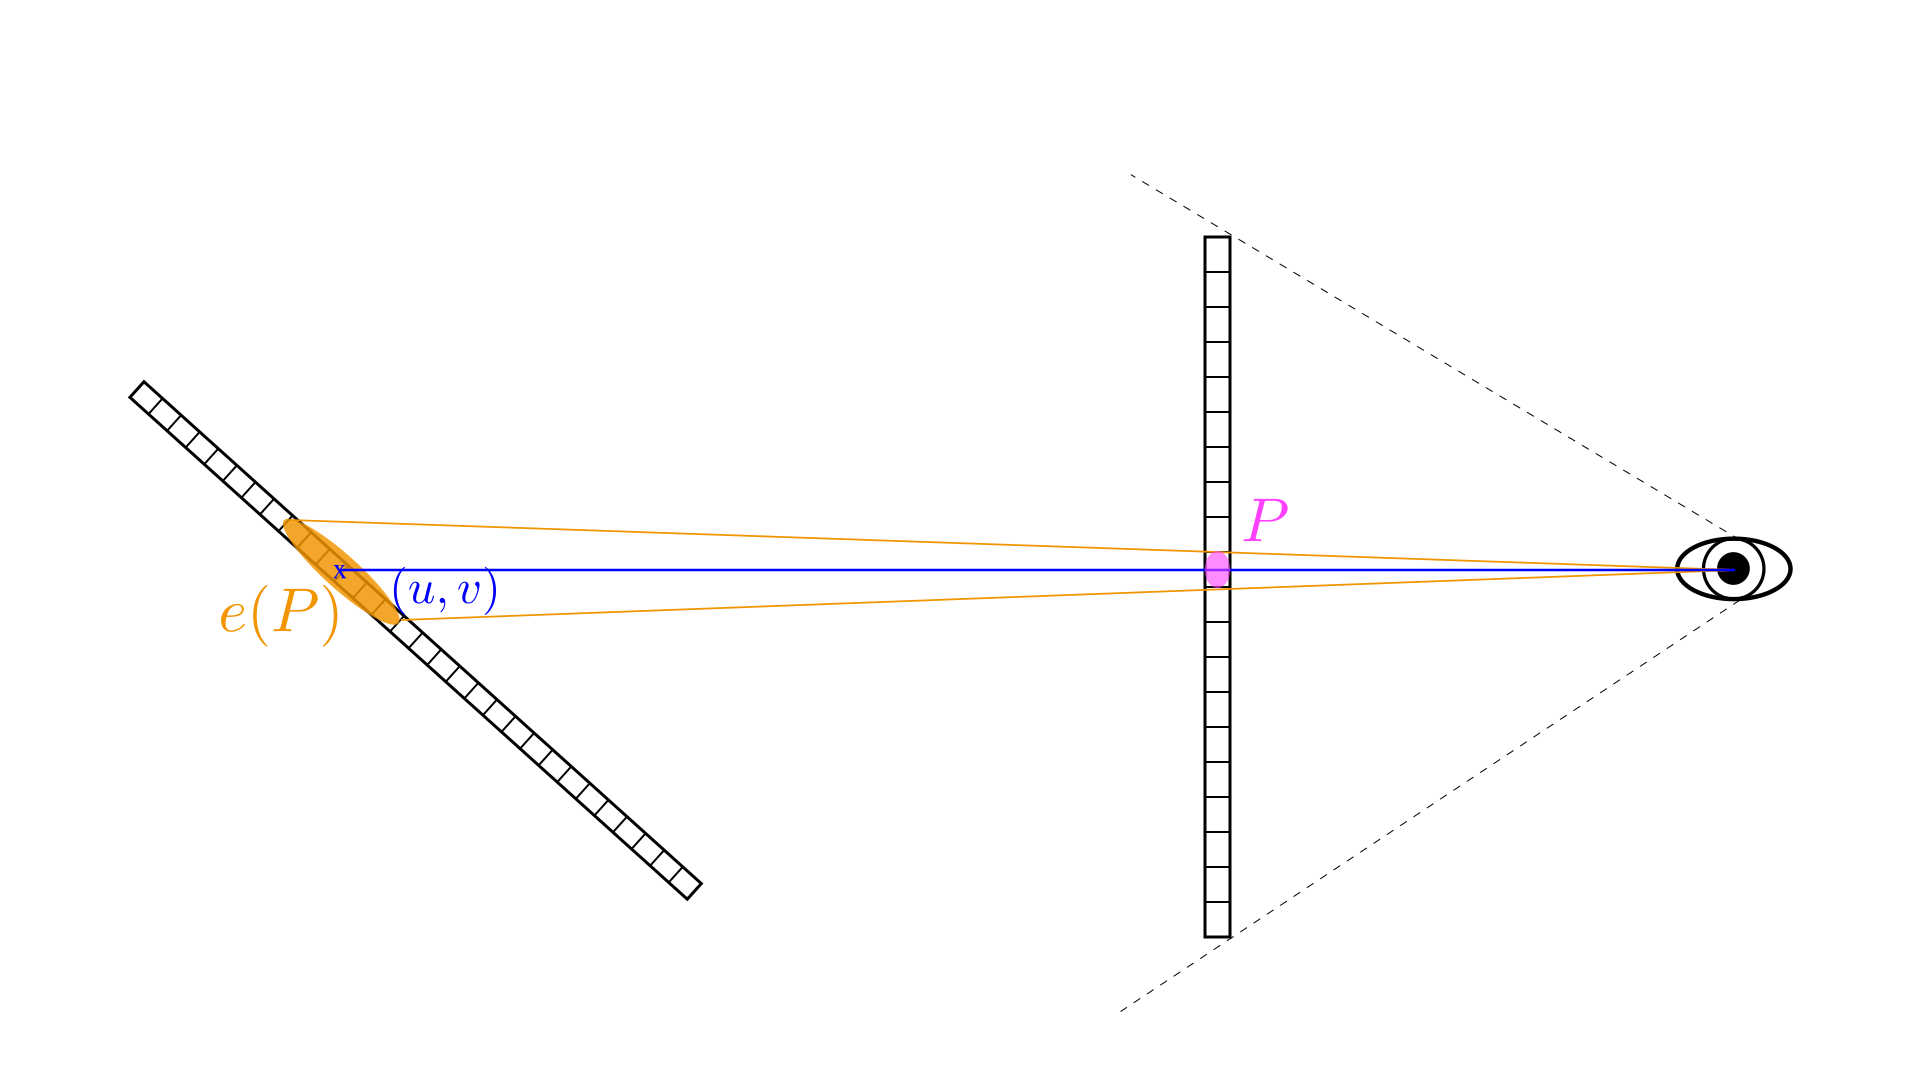
\includegraphics[width=\textwidth]{contenu/resources/images/schema_filtrage}
    \caption[Visualisation du problème d'échantillonnage lors du rendu par rastérisation]{À cette distance de l'écran, l'empreinte $e(P)$ du fragment sur la surface texturée couvre plusieurs texels. Les coordonnées $(u, v)$ ne sont pas suffisantes pour capturer toute l'information de la texture.}
    \label{fig:aliasing}
\end{figure}

Les comportements indésirables causés lors des étapes de rendu et observables sur l'image finale sont appelés artefacts de visualisation. Dans le cas de l'échantillonnage, les artefacts causés par la différence de taille entre un fragment et son empreinte sur une surface texturée sont appelés artefacts d' aliassage. Pour résoudre les problèmes d'aliassage, plusieurs méthodes dites de filtrage sont utilisées, dépendamment du problème d'aliassage rencontré :

\begin{itemize}
    \item le sur-échantillonnage signifie que l'empreinte d'un fragment est plus petite qu'un texel. En cas de sur-échantillonnage, plusieurs fragments voisins peuvent prendre la même valeur. Avoir une même valeur pour plusieurs fragments voisins donne un aspect crénelé à l'image et les contours des objets sont en escalier. La solution idéale dans ce cas est d'augmenter la résolution de la texture utilisée ; ce n'est cependant pas tout le temps possible. Une alternative commune est de faire l'interpolation des valeurs des quatre texels voisins. La texture est échantillonnée quatre fois pour chaque fragment et l'image prend un aspect légèrement flouté, mais l'effet escalier est réduit. Un exemple est montré à la figure~\ref{fig:filtering}
    \item le sous-échantillonnage indique que l'empreinte d'un fragment est plus grande qu'un texel et en recouvre plusieurs, comme à la figure~\ref{fig:aliasing}. En cas de sous-échantillonnage, des fragments voisins représentent du contenu éloigné spatialement sur la surface. La surface entre les centres des empreintes de fragments voisins est alors mal représentée. De loin, la surface texturée présente des motifs dits de moiré. Des bandes non-présentes dans la texture apparaissent sur le rendu et il y a un effet de scintillement lorsque la caméra est déplacée dans la scène. L'apparence souhaitée est l'intégrale des texels qui sont sous l'empreinte du fragment, mais un algorithme de rastérisation naïf ne lit qu'un seul texel. La solution idéale serait de calculer l'intégrale sur tous les texels couverts par l'empreinte du fragment. Calculer l'intégrale directement est souvent irréalisable. L'approche traditionnelle dite filtrage tri-linéaire consiste à pré-calculer une approximation de l'intégrale pour différentes tailles d'empreintes et trouver le bon niveau au moment du rendu. Cette approche double l'occupation mémoire pour chaque texture, mais les effets de moiré disparaissent.

%    \item Différentes résolution des textures utilisées appelées MIPs maps sont pré-calculées avant le rendu. Ces MIPs maps sont l'approximation des intégrales de régions de texels de différentes tailles. La technique de filtrage dit tri-linéeaire consiste à trouver les niveaux adéquats de MIPs maps auquel l'empreinte du fragment a une taille similaire à un texel. L'échantillonnage de la texture se fait alors dans les deux niveaux les plus proches.
%    \item L'alternative classique consiste à pré-calculer différentes échelles de la texture utilisée, appelées MIP maps, et de trouver l'échelle adéquate de telle sorte qu'un texel ait la même taille qu'un fragment. L'échantillonnage est plus lourd et on prend plus d'espace mémoire pour stocker les MIP maps, mais la texture est mieux rendue de loin.
\end{itemize}

\bigskip

\begin{figure}
    \centering
    \begin{subfigure}[b]{.45\textwidth}
        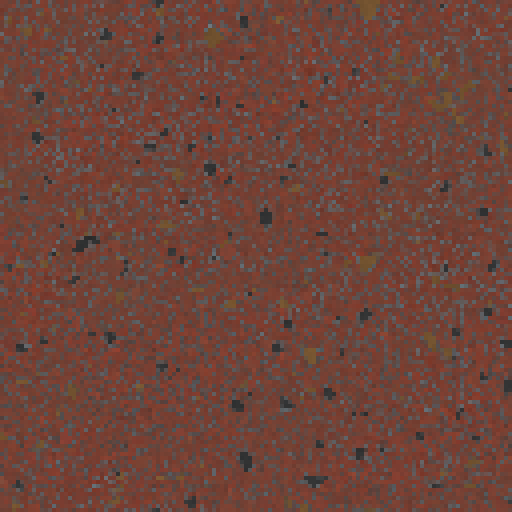
\includegraphics[width=\textwidth]{contenu/resources/images/porcelain_no_filter}
        \caption{Sans filtrage}
    \end{subfigure}
    \hfill
    \begin{subfigure}[b]{.45\textwidth}
        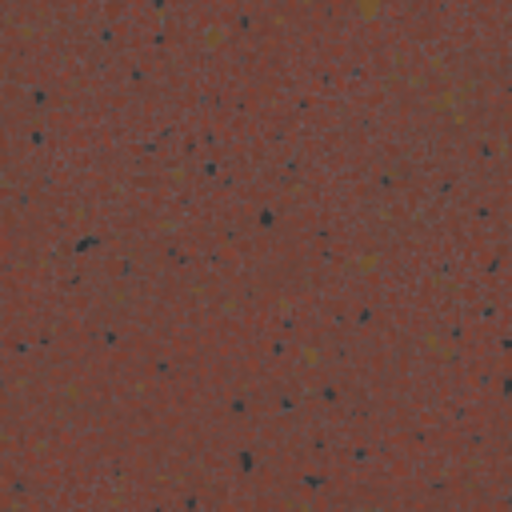
\includegraphics[width=\textwidth]{contenu/resources/images/porcelain_filter}
         \caption{Avec filtrage linéaire}
     \end{subfigure}
    \caption{Filtrer correctement est un enjeu majeur dans l'utilisation des textures}
    \label{fig:filtering}
\end{figure}

S'assurer de filtrer correctement lors de l'échantillonnage est un enjeu majeur pour obtenir un rendu fidèle aux textures utilisées. C'est particulièrement le cas lors la création de textures procédurales, qui est le sujet de cette étude. Diverses méthodes peuvent être utilisées pour la création de textures procédurales. S'assurer de la filtrabilité d'une méthode de création de textures est une des problématiques principales et un critère de qualité de la synthèse de texture, présentée dans la section suivante.

%{\color{red}Pertinence de ce paragraphe ?}
%De nombreuses méthodes de filtrage plus élaborées sont employées pour obtenir des résultats de meilleure qualité, ou pour filtrer des textures plus compliquées. Par exemple quand les textures ne sont plus des images prédéterminées à l'avance, mais qu'elles sont générées au moment du rendu.
% oui pertinent, mentionner les autres solutions "idéales" mais plus difficiles (voir not). filtre analytique et pré-intégration
%OU p-e supprimer paragraphe

\section{Synthèse de texture}

De nombreuses surfaces texturées lors d'un rendu, comme des sols, sont de grande taille. Comme discuté précédemment~\ref{subsec:filtering}, produire des textures de résolution suffisante pour texturer de grandes surfaces sans artefacts demande une grande occupation mémoire et un long temps de création. Étirer les textures en utilisant les coordonnées UV est une solution, qui atteint cependant ses limites assez rapidement. Utiliser une texture de plus basse résolution cause des artefacts visuels. Il est possible de résoudre le problème en créant directement une texture de taille adaptée à la surface à couvrir, procédé appelé synthèse de texture. Par extension, une texture générée par un algorithme de synthèse est aussi appelée une synthèse. Les textures représentent des apparences visuelles de matériaux diverses. Il est possible de classifier des textures de plusieurs manières différentes. Une façon commune de classifier des textures est d'opposer les textures stochastiques, dont les couleurs de pixels semblent aléatoires, et les textures régulières, qui présentent une répétition régulière de motifs~\cite{liu_near-regular_2004}.

\subsection*{Notion de structure}
\label{subsec:structure}

Le travail présenté dans ce manuscript s'intéresse cependant à la synthèse de texture présentant de la structure. Le concept de structure, bien que visuellement intuitif, est difficile à définir de manière formelle. Dans le cadre de ce manuscript, la structure d'une texture désigne comment les différentes parties de la structure sont agencées les unes par rapport aux autres. Dans une texture structurée, les éléments de la texture forment certains schémas ou présentent une certaine forme de régularité. La classification de textures utilisée dans ce travail est faite selon le niveau de structure des textures car c'est le thème central de l'étude. La figure~\ref{fig:échelle-structure} illustre la classification proposée.

\bigskip

\begin{figure}[hb]
    \centering
    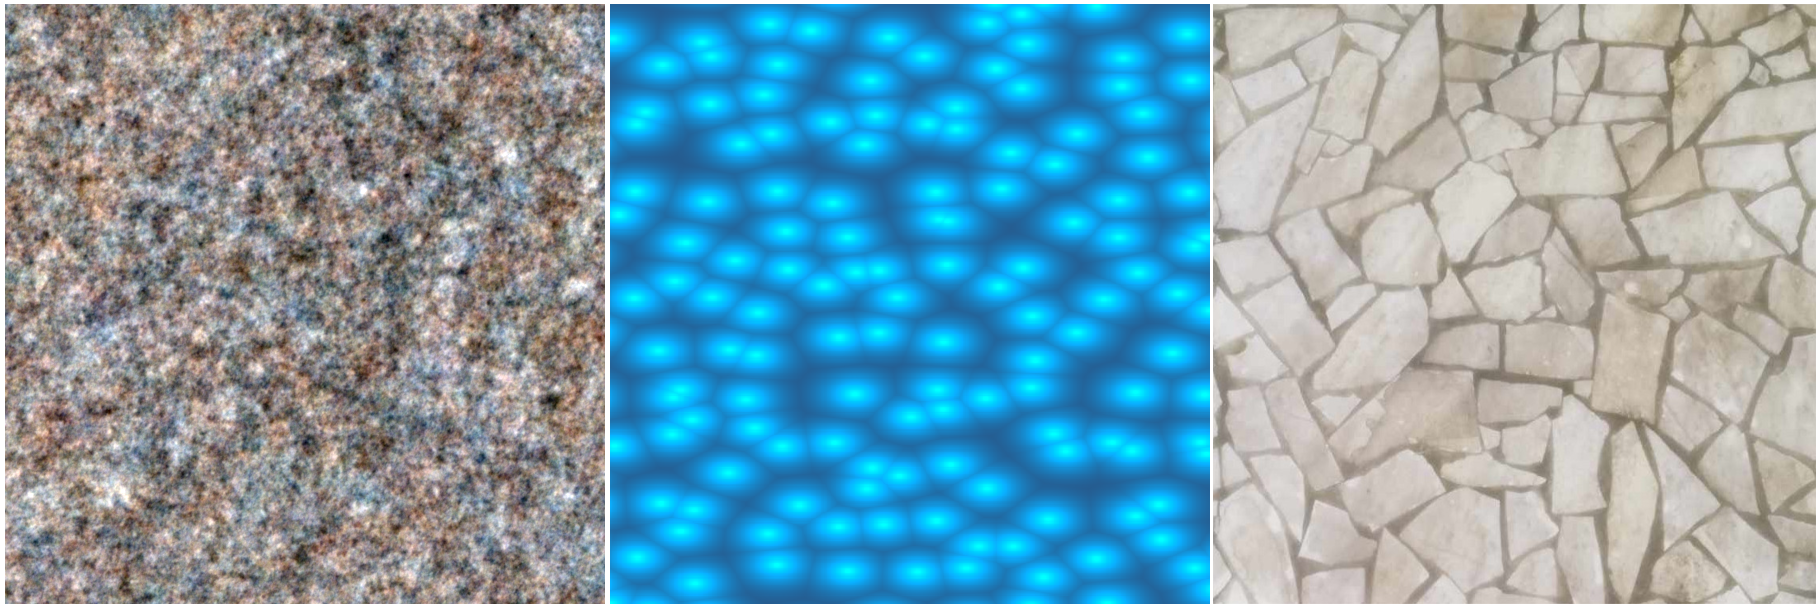
\includegraphics[width=\textwidth]{contenu/resources/images/structure_scale_loucas}
    \caption[Classification des textures selon leur niveau de structure]{Les textures peuvent être classées selon leur niveau de structure : stochastiques ou gaussiennes (gauche), semi-régulières (milieu), ou structurées (droite)}
    \label{fig:échelle-structure}
\end{figure}

L'agencement des éléments de la texture peut se faire à différents niveaux d'échelle. Il y a donc différents niveaux de structure dans une image, principe illustré à la figure~\ref{fig:structure-level}. Les caractéristiques d'une texture telles que l'agencement sont déterminées par des relations statistiques entre les texels de la texture. Préserver toutes les relations statistiques entre les texels est désirable pour la conservation de l'apparence, mais certaines sont trop complexes à préserver en temps-réel. Comprendre quelles relations statistiques préserver et à quel niveau de structure œuvrer sont des enjeux majeurs pour la synthèse de texture structurée et sont l'objet de ce travail.

\begin{figure}[ht!]
    \centering
    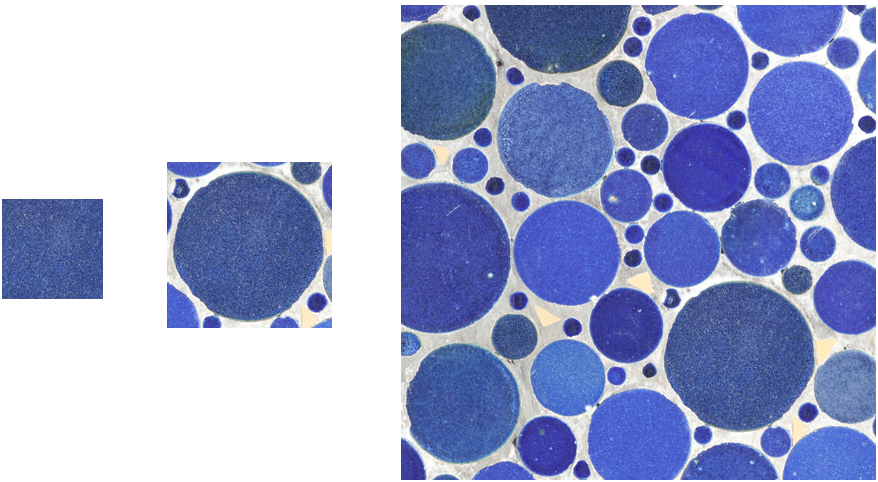
\includegraphics[width=.85\linewidth]{contenu/resources/images/structure_level}
    \caption{Différents niveaux de structure au sein d'une image}
    \label{fig:structure-level}
\end{figure}

\subsection*{Algorithme de synthèse}

Une synthèse de texture un procédé qui permet de produire une texture de taille arbitraire, pouvant prendre en argument des paramètres de différente nature. Différentes synthèses possèdent différentes propriétés, qui peuvent être voulues ou non en fonction de la scène à rendre. Par exemple la texture générée est souvent infinie, il est possible de l'appliquer à des surfaces de taille quelconque avec la résolution désirée. De plus, la texture est évaluée au vol (pendant le rendu) et n'a pas besoin d'être stockée en mémoire. Cela réduit l'occupation mémoire de la texture.

\bigskip

Il existe plusieurs types de synthèses différentes, qui produisent des types de textures différentes. Une première distinction majeure qui est souvent faite est, comme pour le rendu, entre une synthèse hors-ligne et une synthèse en temps réel. Les ressources en temps et en puissance de calcul impliquées diffèrent, les enjeux ne sont pas les mêmes. Les travaux proposés étudient le rendu et la synthèse temps-réel, les synthèses hors-lignes comme les synthèses par optimisation ou par apprentissage profond ne seront pas abordées. Les algorithmes étudiés ici ont la contrainte de devoir s'exécuter au vol, sans que le budget de temps du rendu dépasse le seuil établi. Pour rentrer dans ces contraintes de temps, les méthodes de synthèse exploitent la puissance des cartes graphiques, notamment leur aspect hautement parallélisable. Les algorithmes de synthèse doivent s'exécuter de manière parallèle et chaque fragment doit se calculer indépendamment de ses voisins.

\subsection*{Synthèse temps-réel} % / Types de synthèse

Sous ces contraintes d'efficacité et de rapidité, de nombreux algorithmes subsistent ; deux grandes catégories de méthodes courantes sont la synthèse par réorganisation et la synthèse par convolution.

\subsubsection{Synthèse par réorganisation}

Le but d'une synthèse par réorganisation est de reproduire un extrait de texture donné en entrée en réutilisant et réagençant son contenu. Dans une synthèse par réorganisation, le contenu est découpé en petites régions connexes dites « tuiles ». Plusieurs paramètres comme la taille, forme et disposition des tuiles peuvent être modifiés pour varier la synthèse. L'exemple le plus simple de synthèse par réorganisation est le pavage périodique. Dans un pavage périodique, la texture d'entrée est simplement répétée jusqu'à couvrir la surface désirée. Pour pouvoir faire un pavage périodique, il faut que la texture d'entrée soit périodique, c'est-à-dire qu'elle se répète sans coupure. Le pavage périodique, bien que très rapide, est de faible qualité. Des artefacts visuels sont induits, car il n'y a aucune variation au sein de la texture générée et les motifs sont répétés très régulièrement. Quelques exemples d'artefacts visuels causés par un pavage périodique sont montrés à la figure~\ref{fig:periodic-tiling}. Certains motifs dits saillants sont particulièrement visibles et attirent l'œil, à cause de leur couleur ou de leur forme par exemple. La répétition régulière de motifs saillants n'existe en général pas dans la nature, elle attire encore plus le regard d'une personne observatrice et réduit la sensation d'immersion dans la scène.

\bigskip

\begin{figure}
    \centering
    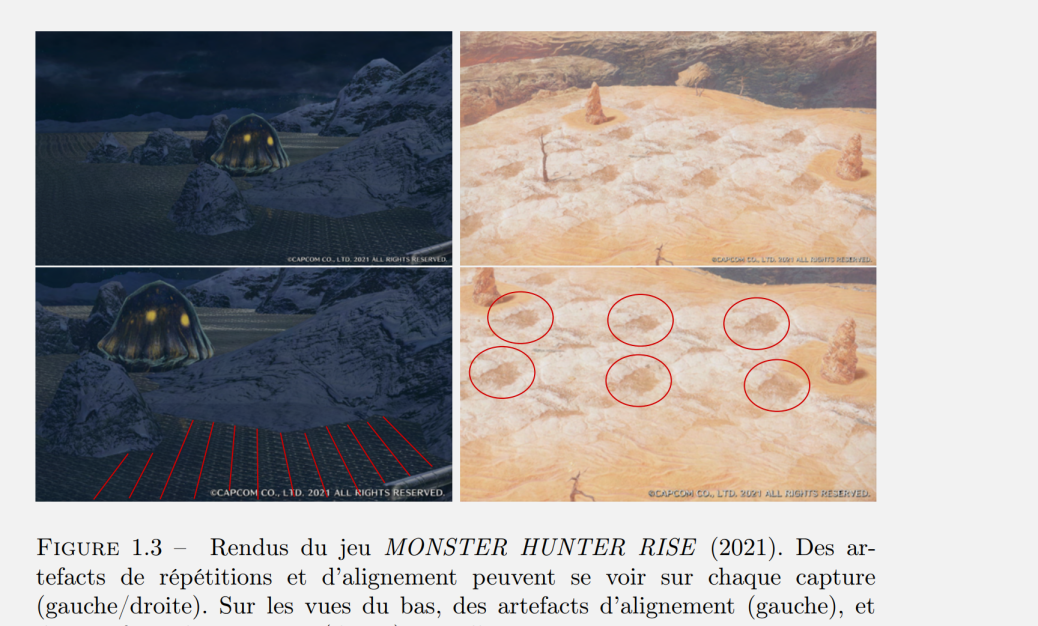
\includegraphics[width=\textwidth]{contenu/resources/images/periodic_tiling}
    \caption[Artefacts d'alignement créés par le pavage périodique]{Artefacts d'alignement créés par le pavage périodique, \textit{Monster Hunter Rise} (2021), Capcom. Crédit à \textit{Nicolas Lutz}~\cite{lutz_processus_2021} pour l'image.}
    \label{fig:periodic-tiling}
\end{figure}

La gestion de l'équilibre entre cohérence et variété est un enjeu majeur dans la synthèse par réorganisation. La cohérence qualifie comment la synthèse reproduit l'apparence visuelle de l'exemple. La variété est la capacité à générer de la nouveauté dans le contenu généré. L'objectif de la synthèse est de propager une apparence similaire à l'exemple sur une grande surface, comme si l'apparence entière avait été synthétisée directement par un unique procédé. Une bonne synthèse doit ainsi apporter à la fois de la cohérence et de la variété. Le pavage périodique par exemple est très cohérent, mais n'apporte aucune variété. Dans un pavage périodique, la tuile qui est réagencée est en fait la texture entière.

\bigskip

Le faible qualité du pavage périodique illustre l'importance du choix de la taille de tuile dans la gestion de l'équilibre entre cohérence et variété. Une grosse tuile capture bien l'apparence de la texture, mais reproduit des motifs saillants qui causent des artefacts et n'offrent pas beaucoup de variété. À l'inverse avec une petite tuile, seulement quelques texels sont réutilisés et certaines relations entre texels éloignés sont perdues, ce qui cause une perte de cohérence. Il est préférable de prendre des tuiles plus petites et mieux les mélanger~\cite{heitz_high-performance_2018} afin de d'obtenir de la variété et d'éviter la répétition de motifs saillants.


\subsubsection{Synthèse par convolution}

L'objectif d'une synthèse par convolution est de construire une texture en disposant des motifs dits noyaux selon une distribution statistique. Un noyau est un petit élément de surface qui peut être un contenu de l'exemple ou du défini de manière fonctionnelle. Le choix du noyau, de la distribution, ainsi que de la méthode de mélange, sont les paramètres à ajuster pour contrôler la synthèse. Une pratique habituelle de la synthèse par convolution est de choisir comme noyau une somme d'ondelettes (typiquement des cosinus) spatialement contraintes et à orientation aléatoire, et de contrôler les fréquences des ondelettes utilisées~\cite{tricard_procedural_2019}. En sélectionnant les fréquences des noyaux, il est possible de contrôler le contenu fréquentiel de la texture synthétisée. Avoir un contrôle sur le contenu fréquentiel de la texture est une bonne méthode pour maîtriser l'apparence de la synthèse~\cite{gilet_local_2014}, comme montré en figure~\ref{fig:lrpn}.

\bigskip

\begin{figure}
    \centering
    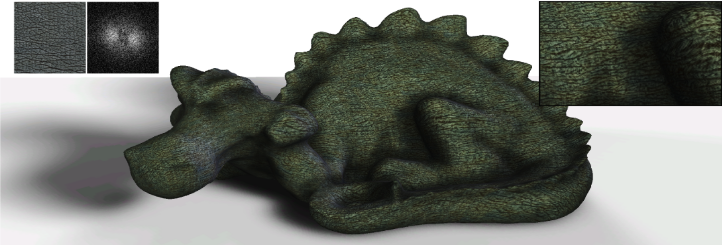
\includegraphics[width=.8\textwidth]{contenu/resources/images/lrpn}
    \caption[Maîtriser le contenu fréquentiel permet de contrôler l'apparence d'une synthèse]{Texture synthétisée par \textit{Local Random Phase Noise}. En approximant le spectre de puissance de l'exemple, Gilet \textit{et al.}~\cite{gilet_local_2014} ont montré que l'apparence de l'exemple est mieux reproduite.}
    \label{fig:lrpn}
\end{figure}

Cependant, la synthèse de texture comportant de la structure en temps-réel est encore un sujet difficile. Les méthodes existantes de synthèse ne fonctionnent pas lorsque la cible contient des motifs organisés ou de la répétition. Quand des méthodes traditionnelles de synthèse temps-réel sont utilisées sur des textures structurées, des artefacts visuels apparaissent. La figure~\ref{fig:synthesis-failure} montre quelques cas d'échec de synthèses de la littérature appliquées aux textures structurées. Il est difficile de créer du contenu réellement nouveau et préservant le même genre de motifs structurés que ceux de l'exemple, car la synthèse cohérente de structure n'est pas encore possible. Certaines configurations présentant des caractéristiques particulières facilitent le problème. Lutz \textit{et al.} ont par exemple montré que la synthèse est possible pour des textures dont la structure est régulière~\cite{lutz_cyclostationary-gaussian_2021}. Le cadre général reste néanmoins non résolu.

\begin{figure}
    \centering
    \begin{subfigure}{.45\textwidth}
        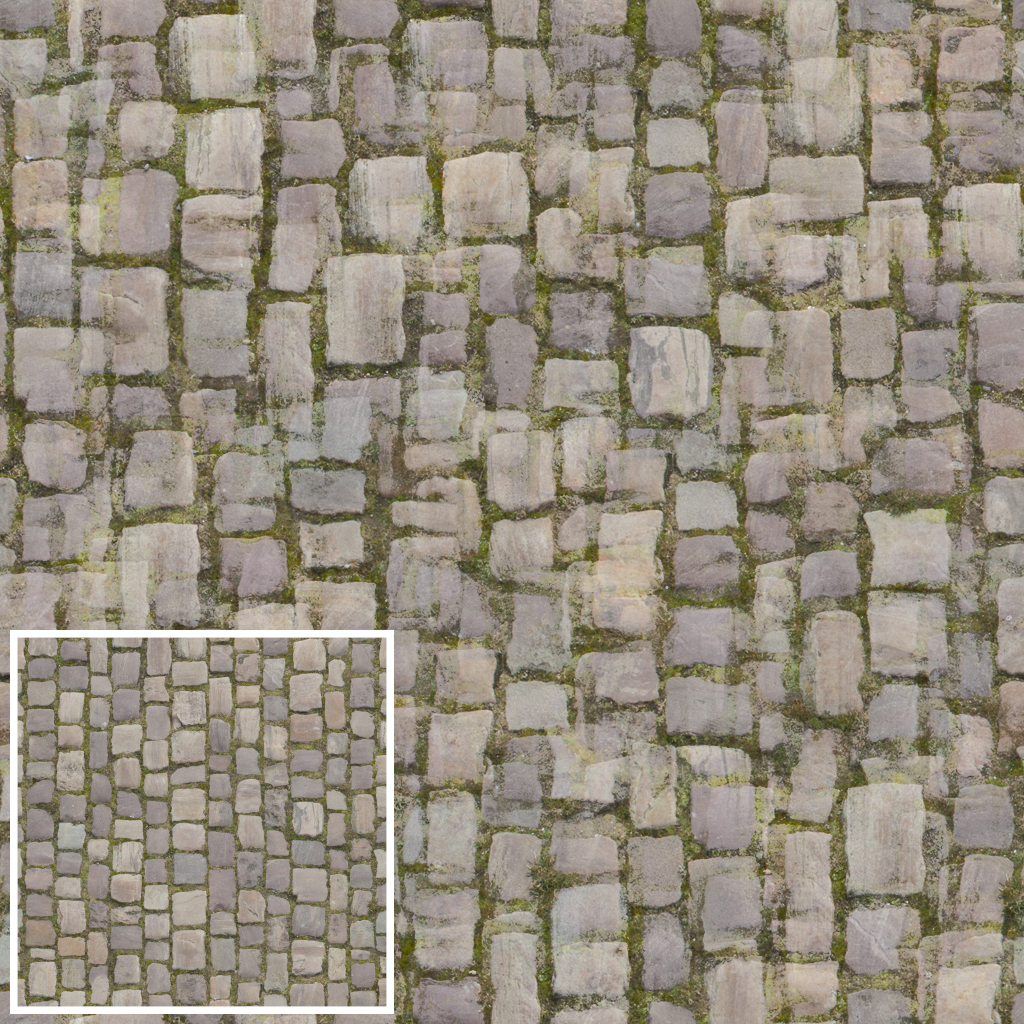
\includegraphics[width=\textwidth]{contenu/resources/images/hpn_failure}
        \caption{Synthèse par pavage et mélange~\cite{heitz_high-performance_2018}.}
    \end{subfigure}
    \hfill
    \begin{subfigure}{.45\textwidth}
        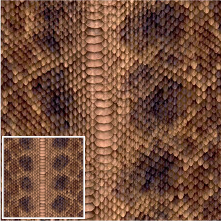
\includegraphics[width=\textwidth]{contenu/resources/images/acf_preserving_hpn_failure}
        \caption{Synthèse préservant la fonction d'autocovariance~\cite{lutz_preserving_2023}.}
    \end{subfigure}

    \caption[Échec de synthèse de texture structurée]{Échec de synthèse de texture structurée. Les méthodes de synthèse actuelles ne sont pas capables de reproduire des textures structurées.}
    \label{fig:synthesis-failure}
\end{figure}

\section{Analyse locale multirésolution}

Un enjeu pour synthétiser des textures structurées est de mieux comprendre ce qui compose la structure d'une texture. Pour comprendre la structure d'une texture, l'idée explorée dans cette recherche est d'appliquer des outils de l'analyse d'image à des processus de synthèse. Les outils choisis permettent l'extraction de caractéristiques d'une texture par l'analyse de relations statistiques inter-texels.

\subsection*{Congruence de phases}

Dans une image, une discontinuité de luminosité est appelée un bord~\cite{torre_edge_1986}. La luminosité ou intensité lumineuse mesure la capacité d'une surface à éclairer dans une certaine direction. En informatique graphique, la luminosité désigne une quantité de lumière présente dans une image. Il a été observé qu'une discontinuité dans la luminosité correspond fréquemment à une discontinuité de la profondeur, de l'orientation, de la reflectance ou de la luminance~\cite{lindeberg_edge_1998}. Les bords d'une image sont donc en lien avec les caractéristiques physiques de la scène représentée. Les bords peuvent représenter une région frontière entre un objet et un autre élément de l'image, comme l'arrière-plan ou un autre objet.

\bigskip

\begin{figure}[h]
    \centering
    \begin{subfigure}[b]{.45\textwidth}
        \centering
        
\includegraphics[width=\textwidth]{contenu/resources/images/discrete_discontinuity}
        \caption{Bord franc}
    \end{subfigure}
    \\
    \vspace{1em}
    \begin{subfigure}[b]{.45\textwidth}
        \centering
        
\includegraphics[width=\textwidth]{contenu/resources/images/discrete_smooth}
        \caption{Bord doux}
    \end{subfigure}
    \caption[Difficulté à définir un bord]{Ces signaux 1D discrets ont des discontinuités en luminosité et représentent un bord. Le premier signal (en haut) a une discontinuité franche, le second (en bas) a une discontinuité floues.}
    \label{fig:edge-difficulty}
\end{figure}

Les bords font partie des éléments qui composent la structure d'une image. Préserver la structure implique donc de préserver les bords. La détection de bords est une tâche difficile car le niveau de discontinuité entre deux texels représentant un bord n'est pas fixé, comme illustré à la figure~\ref{fig:edge-difficulty}. Afin de caractériser les bords et comprendre comment les préserver, il est possible d'utiliser des informations du domaine fréquentiel.

\bigskip

Une image peut être exprimée dans le domaine fréquentiel, ou de Fourier, à l'aide de la transformée de Fourier. Contrairement à la représentation par des texels, dit domaine spatial, l'expression dans le domaine fréquentiel permet de séparer les composantes de l'image selon leur fréquence. La transformée de Fourier est une transformation linéaire qui permet de passer d'une représentation à l'autre. La représentation d'une image dans le domaine de Fourier est dite représentation fréquentielle. Une décomposition dans le domaine fréquentiel permet d'extraire de l'information sur des caractéristiques de l'image qui ne sont pas visibles dans le domaine spatial~\cite{strumillo_fourier}. En particulier Oppenheim a montré que des informations sur la structure d'une image se trouvent dans la phase de sa représentation fréquentielle~\cite{oppenheim_importance_1981}. Morrone \textit{et al.} ont mis au point un modèle physiologiquement réaliste d'énergie locale~\cite{morrone_feature_1987, morrone_feature_1988} qui permet d'extraire des informations sur les éléments saillants d'une image en utilisant la phase. Leur modèle postule que les éléments caractéristiques sont présents dans une image là où les composants de Fourier sont maximalement en phase. Morrone \textit{et al.} introduisent la congruence de phases, grandeur qui quantifie l'alignement de phase des composants de Fourier.

\bigskip

\begin{figure}[h]
    \centering
    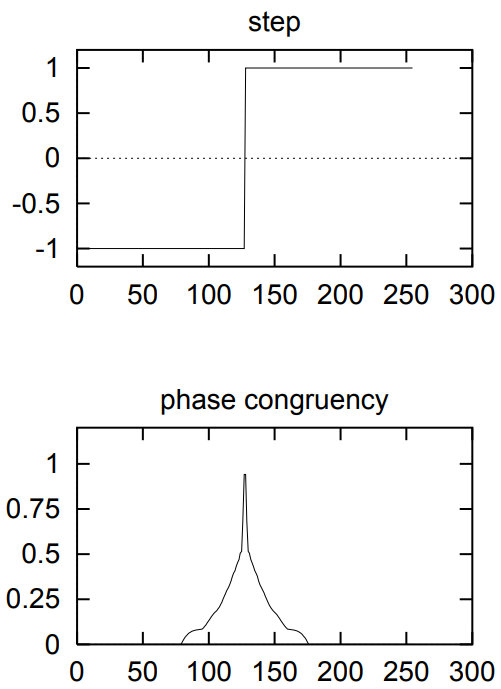
\includegraphics[width=.35\linewidth]{contenu/resources/images/pc_1d_kovesi}
    \caption[Congruence de phases pour un signal 1D]{Congruence de phases pour un signal 1D, Kovesi (1995)~\cite{kovesi_image_1995}}
    \label{fig:pc-1D-kovesi}
\end{figure}

Le travail présenté dans ce manuscript s'intéresse à la congruence de phases comme un moyen d'aider la création de nouvelle structure lors de la synthèse d'une texture. L'objectif est de créer de la structure en introduisant de l'aléatoire, mais de contrôler le processus à l'aide de la congruence de phases. L'étude s'appuie sur les travaux de Kovesi~\cite{kovesi_image_1995}, qui a étendu le modèle de Morrone \textit{et al.}~\cite{morrone_feature_1987, morrone_feature_1988} pour extraire de l'information locale des images~\ref{fig:pc-1D-kovesi}. Une des limites de la transformée de Fourier est en effet que l'information obtenue est spatialement globale. La représentation fréquentielle d'une image ne donne pas directement d'informations sur les relations locales entre les texels. C'est le modèle de Kovesi qui est repris et modifié dans ce travail pour extraire de l'information locale des images. Le modèle de Kovesi est redéfini à l'aide d'un outil mathématique appelé trasnformée de Riesz. La transformée de Riesz permet une représentation alternative d'un signal, avec des informations locales. L'image est ré-exprimée dans un espace différent qui facilite l'étude des relations locales entre les texels.

\subsection*{Analyse multi-échelle}

Comme expliqué précédemment, la structure d'une image est composée de plusieurs niveaux d'échelle. Le travail décrit dans ce manuscrit a pour objectif de synthétiser de la nouvelle structure en préservant certains niveaux de structure et en ajoutant de l'aléatoire à d'autres. Un but de la méthode présentée ici est de pouvoir agir avec précision sur certains niveaux d'échelle de structure ciblés. Une méthode d'analyse qui permet de travailler avec plusieurs niveaux de résolution d'une même image est dite multirésolution~\cite{mallat_theory_1989}, ou multi-échelle. Des exemples d'application communs de méthodes d'analyse multirésolution sont la détection robuste de caractéristiques de différentes tailles~\cite{park_multiresolution_2010} et la compression d'images~\cite{averbuch_image_1996}. Dans cette étude, l'analyse multirésolution est faite à l'aide d'une pyramide d'images. Une pyramide d'images est une méthode de représentation d'image qui permet d'étudier les différences de détails entre les différents niveaux d'échelle.

\section{Plan du manuscript} % / problématique

Ce manuscrit est organisé comme suit :

\begin{itemize}
%    \item revue de l'état de l'art de la synthèse de texture temps réel,
    \item explication de la théorie de Riesz et du modèle d'analyse locale multi-échelle qui en découle,
    \item application à la synthèse de texture par échantillonnage préférentiel.
\end{itemize}